% Chapter Template

\chapter{Approach and direct formulation of noise analysis} % Main chapter title
\label{approach} % Change X to a consecutive number; for referencing this chapter elsewhere, use \ref{ChapterX}

\lhead{\emph{Approach and direct formulation of noise analysis}} % Change X to a consecutive number; this is for the header on each page - perhaps a shortened title

%----------------------------------------------------------------------------------------
%	SECTION
%----------------------------------------------------------------------------------------
\section{Direct formulation of noise analysis} \label{direct_approach}
The intention behind this study is to perform a flow field noise analysis in CFD without implementation of acoustical analogies to the CFD code itself. Moreover, very limited information on direct formulation of noise analysis was found during the research, with even fewer research on acoustical near field of transonic axial compressors or axial fans of twin spool jet engines.

The process for the direct formulation noise analysis is following:
\begin{enumerate}
\item Obtain raw flow field data of static pressure, velocity magnitude from CFD analysis.
\item Perform averaging over time of pressure and velocity magnitude for each point or cell in the flow field (equation \ref{eq:avg}).
\item Obtain offset from mean static pressure and velocity magnitude for every timestep for every point/cell in the saved flow field (equation \ref{eq:off}).		
\end{enumerate}

%The process purposely omits transformation of pressure to complex form and forces the analysis on direct signal as measured by a pressure sensor.

\begin{equation} \label{eq:avg}
\bar{p} = \frac{1}{n} \sum_{n=1}^{N} p_k \qquad and \qquad \bar{u} = \frac{1}{n} \sum_{n=1}^{N} u_k
\end{equation}

\begin{equation} \label{eq:off}
p_{n \; sound} = p_n - \bar{p} \qquad and \qquad u_{n \; particle} = u_n - \bar{u}
\end{equation}

Sound pressure signal and flow velocity offset is obtained for every node or cell centroid throughout the simulation flowtime. This dataset can be now post processed. Dataset obtained in described manner now contains sound pressure of the flow field in every mesh node or cell centroid throughout the computational time. The dataset is now post processed to obtain quantity information of the acoustic nearfield. 

Sound intensity for cells/nodes in fluid volume is calculated using formula \ref{eq:sil}. 

\begin{equation} \label{eq:sil}
I_{n} = p_{n \; sound} \cdot u_{n \; particle}
\end{equation}

RMS sound pressure level and intensity level can be obtained from the respective data with use of the formula \ref{eq:RMS}.

\begin{equation} \label{eq:RMS}
p_{rms} = \sqrt{\frac{\sum_{n=1}^{N} p_{n \; sound}^{2}}{N}} \qquad I_{rms} = \sqrt{\frac{\sum_{n=1}^{N} u_{n \; particle}^{2}}{N}}
\end{equation}

Sound pressure decibel level (SPLdB) for time specific $p_{k \; sound}$ values and and RMS values $p_{rms}$ is computed using formula \ref{eq:SPLdB} with standard reference pressure $p_{ref} = 20 \mu Pa$, whereas for sound intensity with formula \ref{eq:SILdB} and with reference intensity $I_{ref} = 1 pW/m^{2}$.

\begin{equation} \label{eq:SPLdB}
SPLdB = 20 \cdot \log_{10}\left(\frac{|p_{n \; sound}|}{p_{ref}}\right)
\end{equation}

\begin{equation} \label{eq:SILdB}
SILdB = 10 \cdot \log_{10}\left(\frac{|I_{n}|}{I_{ref}}\right)
\end{equation}

The signal obtained by direct approach is stored in discrete time samples, therefore using a continuous Fourier Transform would require approximation of the sampled signal to a continuous function, which for large datasets is unjustified. In order to obtain ordinary sinuses of the acoustic signal a Discrete Fourier Transform is performed (eq. \ref{eq:dft}).

\begin{equation} \label{eq:dft}
X_k = \sum_{n=0}^{N-1} x_n \cdot e^{-\frac{j2 \pi kn}{N}}
\end{equation}

Let's assume that:

\begin{equation} \label{eq:bn}
b_n = \frac{2 \pi k n}{N}
\end{equation}

Therefore, the equation \ref{eq:dft} can be written as:
\begin{equation} \label{eq:dft2}
X_k = x_{0} e^{-j b_{0}} + x_{1} e^{-j b_{1}} + x_{2} e^{-j b_{2}} + \ldots + x_{n} e^{-j b_{N-1}}
\end{equation}

Using Euler's identity the exponent is decomposed (eq. \ref{eq:euler}) to a complex sum:

\begin{equation} \label{eq:euler}
e^{jx} = \cos(x) + j \cdot \sin(x)
\end{equation}

Therefore the equation \ref{eq:dft} can be written as:

\begin{equation} \label{eq:dft3}
X_k = x_0 [\cos(-b_{0}) + j \sin(-b_{0})] +  \ldots + x_n [\cos(-b_{N-1}) + j \sin(-b_{N-1})]
\end{equation}

Rearranging the equation \ref{eq:dft3} and summing up the real and imaginary components will return a complex vector $X_k$ for "k-th" frequency bin.

\begin{equation} \label{eq:complex}
X_k = A_k + j B_{k}
\end{equation}
 
The frequency resolution of the DFT depends on the sampling frequency and number of samples, and is calculated by formula \ref{eq:samples}. 

\begin{equation} \label{eq:samples}
f_{bin} = \frac{f_{s}}{N}
\end{equation}

Fourier coefficients are then used to compute the amplitude (eq. \ref{eq:dftmag}) and phase shift (eq. \ref{eq:dftphase}) for the "k-th" frequency bin ordinary sinus.

\begin{equation} \label{eq:dftmag}
\text{Amp}_k = 2 \cdot \sqrt{A_{k}^{2} + B_{k}^{2}} \cdot \frac{1}{N}
\end{equation}

\begin{equation} \label{eq:dftphase}
\theta_k = \arctan \frac{B_k}{A_k}
\end{equation}


%-----------------------------------
%	SECTION
%-----------------------------------
\section{CFD analysis requirements} \label{cfdreq}
References \citep{Light1}, \citep{Light2}, \citep{FWH} and \citep{curle} provide a theoretical insight on generating sound in fluid flow due to shear mixing of flows or by implementing a solid boundary in the flow. General remark is: any source of turbulence that result in pressure fluctuation will result in generating sound. Therefore the main requirement for used CFD code for direct noise analysis is the capability of resolving turbulent flow and corresponding fluctuations of the pressure.

Let's consider the effect of injection of energy to the fluid resulting in creation of eddies (Fig. \ref{CFDTypes})

\begin{figure}[h!]
\centering % bo \centering nie wstawia dodatkowego odstępu
\includegraphics[width=0.85\textwidth]{Pictures/CFD_Types.png}
\caption{Resolving eddies in different kinds of CFD analyses}
\label{CFDTypes}
\end{figure}

\subsection{Govering equations} \label{goveq}

Continuity equation:
\begin{equation} \label{eq:cont}
\frac{\partial \rho}{\partial t} + \nabla (\rho U) = 0
\end{equation}

Momentum equation:
\begin{equation} \label{eq:momentum}
\frac{dU}{dt} = - \frac{1}{\rho} \nabla p + \nu \nabla^{2} U
\end{equation}

\subsection{Direct Numerical Simulation} \label{DNS}
Considering the direct formulation of noise, the Direct Numerical Simulation is seemingly the best tool of choice. The DNS formulation of flow solves directly the discrete form of Navier-Stokes Equation without any turbulence models. Size limit of the resolved eddies is the Kolmogorov limit (eq. \ref{eq:kolm}). In order to properly resolve the DNS simulation op to this scale, the mesh sizing must be at least as small as the expected Kolmogorov limit at given Reynolds number.

\begin{equation} \label{eq:kolm}
\eta \approx \frac{l}{Re^{3/4}}
\end{equation}

Reference \citep{LES_size} provides information on calculating the mesh grid node count for DNS calculations (eq. \ref{eq:dnscount}) for flat plate airfoil of aspect ratio $L_z / L_x$. The computational box for this case is of size $L_x \times \delta \times L_z$ in streamwise, normal to plate and spanwise direction respectively, where $\delta$ is the boundary layer thickness.

\begin{equation} \label{eq:dnscount}
N_{DNS} = 0.000153 \frac{L_z}{L_x} Re_{L_x}^{37/14} \left[ 1 - \left( \frac{Re_{x_0}}{Re_{L_x}} \right)^{23/14} \right]
\end{equation}

Point $x_0$ is the location where formulas \ref{eq:delta} and \ref{eq:cf} are valid for Reynolds number range ($10^6 \leq Re_x \leq 10^9$).

\begin{equation} \label{eq:delta}
\delta = x \cdot  0.16 Re_x^{(-1/7)}
\end{equation}

\begin{equation} \label{eq:cf}
c_f = 0.027 Re_x^{(-1/7)}
\end{equation}

For aspect ratio $L_z / L_x = 4$ and $Re_{x_0} = 5 \cdot 10^5$ the node count for streamwise $Re = 10^6$ is roughly $2.99 \cdot 10^{12}$ nodes and for $Re = 10^7$ is roughly $1.92 \cdot 10^{15}$ nodes.

Such node and cell counts are impossible to solve within practical walltime, therefore usage of DNS for sound analysis is limited to small Reynolds numbers.

%Figure \ref{kolmscale} shows the Kolmogorov limit and hence the volume mesh sizing required for the analysis. For Reynolds numbers above 1 million the limit is below $3.1 \cdot 10^{-5}$ meters, for $Re > 10^{7}$ the limit goes below $5.6 \cdot 10^{-6}$ meters. Use of such fine mesh elements generates mesh cell count in order of magnitude of billions for objects like a single passage of the compressor rotor, and hence is plainly impractical to use with high Reynolds numbers.

%\begin{figure}[h!]
%\centering % bo \centering nie wstawia dodatkowego odstępu
%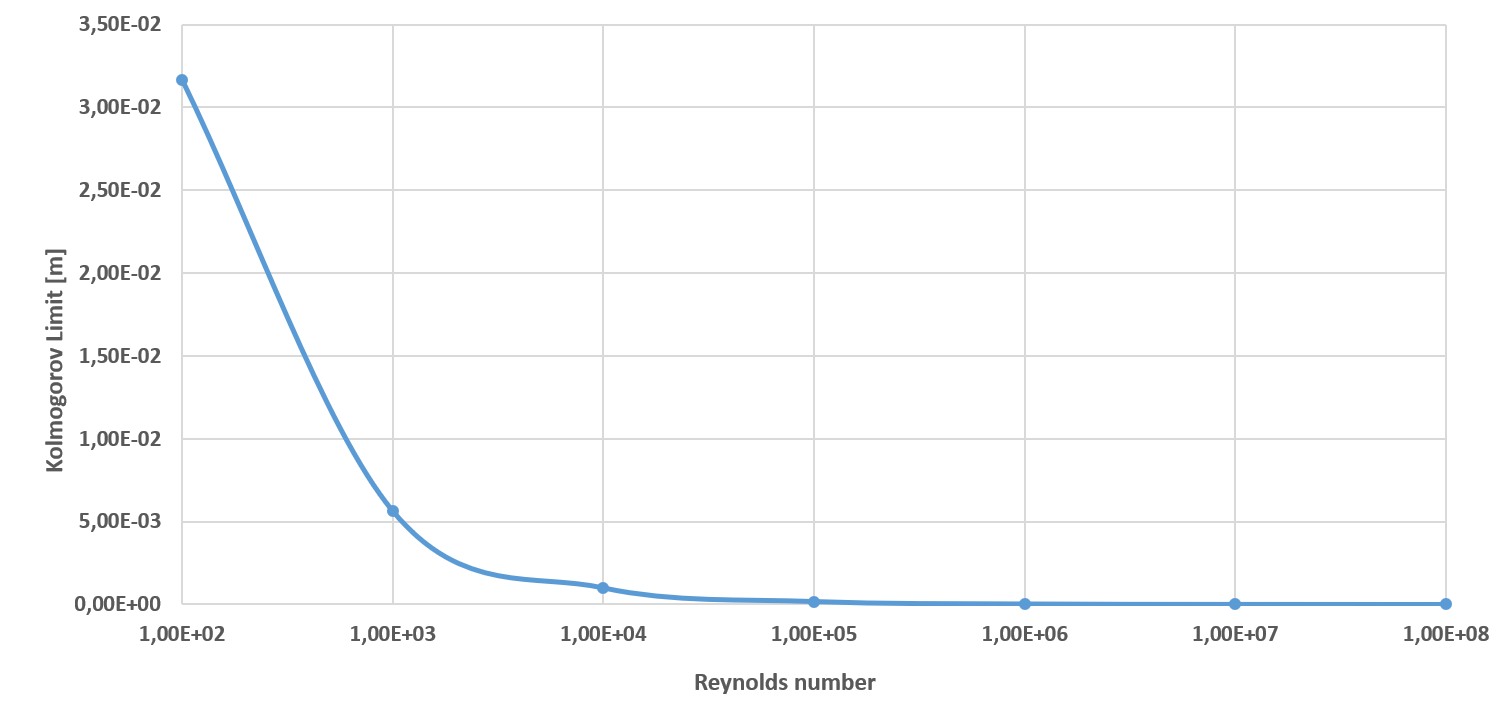
\includegraphics[width=0.85\textwidth]{Pictures/kolm_scale.png}
%\caption{Kolmogorov limit for given Reynolds number}
%\label{kolmscale}
%\end{figure}


\subsection{Large Eddy Simulation} \label{LES}
Large eddy simulation (LES) is a mathematical model for turbulence used in computational fluid dynamics. It was initially proposed in 1963 by Joseph Smagorinsky to simulate atmospheric air currents \citep{LES1}.

The principal idea behind LES is to reduce the computational cost by ignoring the smallest length scales, which are the most computationally expensive to resolve, via low-pass filtering of the Navier–Stokes equations. Such a low-pass filtering, which can be viewed as a time- and spatial-averaging, effectively removes small-scale information from the numerical solution. This information is not irrelevant, however, and its effect on the flow field must be modeled, a task which is an active area of research for problems in which small-scales can play an important role such as acoustics \citep{LES2}.

The governing equations employed for LES are obtained by filtering the time dependent Navier-Stokes equations in either Fourier (wave-number) space or configuration (physical) space. The filtering process effectively filters out the eddies whose scales are smaller than the filter width or grid spacing used in the computations. The resulting equations therefore govern the dynamics of large eddies \citep{fluenttheory}.

A filtered variable is defined by:
\begin{equation} \label{eq:lesfilter}
\overline{\phi}(x) = \int\displaylimits_{D} \phi \left( x' \right) G \left( x, x' \right) dx'
\end{equation}

\noindent where $D$ is the fluid domain, and $G$ is the filter function that determines the scale of the resolved eddies. The finite volume discretization itself implicitly provides the filtering operation:

\begin{equation} \label{eq:lesfilter2}
\overline{\phi}(x) = \frac{1}{V} \int\displaylimits_{\nu} \phi \left( x' \right) dx', \; x' \in \nu
\end{equation}

\noindent where $V$ is the volume of a computational cell. The filter function, $G(x, x')$ implied here is then:

\begin{equation} \label{eq:lesfilter3}
G(x, x') = 
\begin{cases}
	\frac{1}{V}, & \text{if } x'\in \nu \\
	0, & \text{otherwise}
\end{cases}
\end{equation}

For compressible flows, it is convenient to introduce the density-weighted (or Favre) filtering operator:
\begin{equation} \label{eq:favre}
\tilde{\phi} = \frac{\overline{\rho \phi}}{\overline{\phi}}
\end{equation}

Filtering the continuity \ref{eq:cont} and momentum \ref{eq:momentum} equations following form is obtained:

\begin{equation} \label{eq:lescont}
\frac{\partial \rho}{\partial t} + \frac{\partial}{\partial x_i} \left( \rho \overline{u_i} \right) = 0
\end{equation}

\begin{equation} \label{eq:lesmom}
\frac{\partial}{\partial t} \rho \overline{u_i}
+ \frac{\partial}{\partial x_j} \left( \rho \overline{u_i} \overline{u_j} \right)
= \frac{\partial}{\partial x_j} \left( \sigma_{ij} \right)
- \frac{\partial \overline{p}}{\partial x_i}
- \frac{\partial \tau_{ij}}{\partial x_j}
\end{equation}

\noindent where $\sigma_{ij}$ is the stress tensor due to molecular viscosity defined by:

\begin{equation} \label{eq:lesstress}
\sigma_{ij}
\equiv
\left[ \mu \left( \frac{\partial \overline{u_i}}{\partial x_{j}} + \frac{\partial \overline{u_j}}{\partial x_{i}} \right) \right]
- \frac{2}{3} \mu \frac{\partial \overline{u_l}}{\partial x_l} \delta_{ij}
\end{equation}

\noindent and $\tau_{ij}$ is the subgrid-scale stress defined by:

\begin{equation} \label{eq:lessubstress}
\tau_{ij} \equiv \rho \overline{u_i u_j} - \rho \overline{u_i} \; \overline{u_j}
\end{equation}

The Favre Filtered Navier-Stokes equation takes the same form as equation \ref{eq:lesmom}. The compressible form of the subgrid stress tensor is defined as:

\begin{equation} \label{eq:lescompsub}
\tau_{ij} = \overline{\rho} \tilde{u_i u_j} - \overline{\rho} \tilde{u_i} \; \tilde{u_j}
\end{equation}

The subgrid-scale stresses resulting from the filtering operation are unknown, and require modeling. The subgrid-scale turbulence models employ the Boussinesq hypothesis \citep{bousinesque} in the RANS models, computing subgrid-scale turbulent stresses from:

\begin{equation} \label{eq:lesturbstress}
\tau_{ij} - \frac{1}{3} \tau_{kk} \delta_{ij} = -2 \mu_{t} \overline{S_{ij}}
\end{equation}

\noindent where $\mu_t$ is the subgrid-scale turbulent viscosity. The isotropic part of the subgrid-scale stresses $\tau_{kk}$ is not modeled, but added to the filtered static pressure term. $S_{ij}$ is the rate-of-strain tensor for the resolved scale defined by:

\begin{equation} \label{eq:lesstrain}
\overline{S_{ij}} \equiv \frac{1}{2} \left( \frac{\partial \overline{u_i}}{\partial x_j} + \frac{\partial \overline{u_j}}{\partial x_i} \right)
\end{equation}

Equation \ref{eq:lescompsub} is split into its isotropic and deviatoric parts:

\begin{equation} \label{eq:lesdeviatoric}
\tau_{ij} - \frac{1}{3} \tau_{kk} \delta_{ij} = -2 \mu_{t} \left( S_{ij} - \frac{1}{3} S_{kk} \delta_{ij} \right)
\end{equation}

Using LES approach is viable for resolving directly formulated noise, yet the computational cost of such calculations is still relatively large due to mesh sizing requirements. As stated by \citep{LES_size} the required node count for the analysis can be described by formulas \ref{eq:leswm} and \ref{eq:leswr} for modeled and resolved boundary layers.

\begin{equation} \label{eq:leswm}
N_{wm} = 54.7 \frac{L_z}{L_x} n_x n_y n_z Re^{2/7}_{L_x} \left[ \left( \frac{Re_{L_x}}{Re_{x_0}} \right)^{(5/7)} - 1\right]
\end{equation}

\begin{equation} \label{eq:leswr}
N_{wr} = 0.021 \frac{n_y}{\Delta x_w^{+} \Delta z_w^{+}} \frac{L_z}{L_x} Re^{13/7}_{L_x} \left[ 1 - \left( \frac{Re_{L_x}}{Re_{x_0}} \right)^{(6/7)} \right]
\end{equation}

The computational box for this case is of size $L_x \times \delta \times L_z$ in streamwise, normal to plate and spanwise direction respectively, where $\delta$ is the boundary layer thickness.

For $L_z / L_x = 4$ and $Re_{x_0} = 5 \cdot 10^5$ the node count for streamwise $Re = 10^6$ and $Re = 10^7$ is computed. The $n_x n_y n_z$ product is the number of grid points to resolve the cubic computational volume $\delta^3$ exterior to the viscous wall region. Suggested value of $n_x n_y n_z = 2500$, where $n_x = 10 \; n_y = 25 \; n_z = 10$ was used for the computation of node count with equation \ref{eq:leswm}. Suggested $\Delta x_w^{+} \approx 100$, $\Delta z_w^{+} \approx 20$ and $n_y \approx 10$ was used for computation of node count with equation \ref{eq:leswr}.

Node count for $Re = 10^6$ is roughly $1.82 \cdot 10^{7}$ nodes for modelled and $2.61 \cdot 10^{7}$ nodes for resolved wall flow. For $Re = 10^7$ the figures are $4.10 \cdot 10^{8}$ and $3.88 \cdot 10^{9}$ nodes respectively \citep{LES_size}.

It must be noted that provided cell count is solely for a flow box of boundary layer width. Respective mesh sizing should be propagated towards volume of the computational domain thus enlarging the mesh even further.

LES analyses are commonly used in research and engineering and the method used is feasible for the direct noise formulation. However the computational expense of running such cases is high, but manageable. Second limiting factor for LES is the amount of data generated during the process. As the direct approach requires storing at least every second time step for further processing, terabytes of data are predicted.

\subsection{Reynolds Averaged Navier Stokes} \label{RANS}
The most computationally efficient method for resolving turbulent flows is using Reynolsds Averaged Navier Stokes equation. Consider a conservation variable $\phi$ of fluid described by spatial and temporal variables. The quantity may be decomposed to a sum of time averaged value in given spatial coordinates and time dependent fluctuations (eq. \ref{eq:rdecomp}).

%\begin{equation} \label{eq:NS}
%\rho \left(\frac{\partial u_i}{\partial t} + u_j \frac{\partial u_i}{x_j} \right) = - \frac{\partial p}{\partial x_j} + \mu \frac{\partial^2 u_i}{\partial x_j \partial x_j} + \frac{\mu}{3} \frac{\partial^2 u_j}{\partial x_i \partial x_j} + \rho g_i
%\end{equation}

\begin{equation} \label{eq:rdecomp}
\phi (x, y, z, t) = \overline{\phi (x, y, z, t)} + \phi ' (x, y, z, t)
\end{equation}

Consider at first the continuity equation \ref{eq:cont}. By applying Reynolds decomposition to velocity vector we obtain:

\begin{equation} \label{eq:cont_rans1}
\frac{\partial \rho}{\partial t} + \frac{\partial \overline{\rho u_i}}{\partial x_i} + \frac{\partial \rho u'_i}{\partial x_i} = 0
\end{equation}

By averaging the both sides of the equation  \ref{eq:cont_rans1} and applying averaging rules to its components we obtain:

\begin{equation} \label{eq:cont_rans2}
\frac{\partial \rho}{\partial t} + \frac{\partial \overline{\overline{\rho u_i}}}{\partial x_i} + \frac{\partial \overline{\rho u'_i}}{\partial x_i} = 0
\end{equation}

Because the average of an average is equal average, and  the average of the fluctuation component is equal 0 we obtain equation \ref{eq:cont_rans3}, the Reynolds averaged continuity equation.

\begin{equation} \label{eq:cont_rans3}
\frac{\partial \rho}{\partial t} + \frac{\partial \overline{\rho u_i}}{\partial x_i} = 0
\end{equation}

By taking the momentum equation \ref{eq:momentum}, switching to the index notation and applying the Reynolds decomposition we obtain the equation \ref{eq:mom_decomp1}

\begin{equation} \label{eq:mom_decomp1}
\underbrace{\frac{\partial \left( \overline{u_i} + u'_i \right)}{\partial t}}_\text{1} 
+ \underbrace{\left( \overline{u_j} + u'_j \right) \frac{\partial \left( \overline{u_j} + u'_j \right)}{\partial x_j}}_\text{2} 
=
- \underbrace{\frac{1}{\rho} \frac{\partial \left( \overline{p} + p' \right)}{\partial x_i}}_\text{3} 
+ \underbrace{\nu \frac{\partial^2 \left( \overline{u_i} + u'_i \right)}{\partial x_j^2}}_\text{4} 
\end{equation}

Components 1, 3 and 4 of the above equation are treated in the same manner as the continuity equation and thus we obtain:

\begin{equation} \label{eq:mom_components}
\underbrace{\frac{\partial \overline{u_i}}{\partial t}}_\text{1}
\qquad
\underbrace{\frac{1}{\rho} \frac{\partial \overline{p}}{\partial x_i}}_\text{3}
\qquad
\underbrace{\nu \frac{\partial^2 \overline{u_i}}{\partial x_j^2}}_\text{4}
\end{equation}

The decomposition of component 2 from the equation \ref{eq:mom_decomp1} requires multiplication of the components within the braces and performing Reynolds averaging on each of the products: 

\begin{equation} \label{eq:mom_comp2_avg}
\underbrace{\overline {\left( \left( \overline{u_j} + u'_j \right) + \frac{\partial \left( \overline{u_i} + u'_i \right)}{\partial x_j} \right)}}_\text{2}
= \underbrace{\overline{\left( \overline{u_j} \frac{\partial \overline{u_i}}{\partial x_j} \right)}}_\text{M $\cdot$ M $\neq$ 0}
+ \underbrace{\overline{\left( \overline{u_j} \frac{\partial u'_i}{\partial x_j} \right)}}_\text{M $\cdot$ F = 0}
+ \underbrace{\overline{\left( u'_j \frac{\partial \overline{u_i}}{\partial x_j} \right)}}_\text{F $\cdot$ M = 0}
+ \underbrace{\overline{\left( u'_j \frac{\partial u'_i}{\partial x_j} \right)}}_\text{F $\cdot$ F $\neq$ 0}
\end{equation}

The F $\cdot$ F $\neq$ 0 product can be further simplified by equation:

\begin{equation} \label{eq:ff}
\frac{\partial u'_j u'_i}{\partial x_j}
= \underbrace{u'_j \frac{\partial u'_j}{\partial x_j}}_\text{= 0}
+ \underbrace{u'_j \frac{\partial u'_i}{\partial x_j}}_\text{F $\cdot$ F $\neq$ 0}
\end{equation}

By inserting the components 1 through 4 from equations \ref{eq:mom_components} and \ref{eq:mom_comp2_avg} modified by equation \ref{eq:ff} to the equation \ref{eq:mom_decomp1} we obtain the Reynolds averaged momentum equation:

\begin{equation} \label{eq:RANSmomentum}
\frac{d \overline{U}}{dt}
=
- \frac{1}{\rho} \frac{\partial \overline{p}}{\partial x_i}
+ \frac{\partial}{\partial x_j} \left[ \nu \frac{\partial \overline{u_j}}{\partial x_j} - \overline{u'_i u'_j}\right]
\end{equation}

By representing the viscous terms as a stress tensor (eq. \ref{eq:viscous}) we obtain the momentum equation with turbulent stress (eq \ref{eq:RANSmomentum2})

\begin{equation} \label{eq:viscous}
\nu \frac{\partial^2 \overline{u_i}}{\partial x_j^2}
=
\frac{1}{\rho} \frac{\partial}{\partial x_j} \tau_{ij}
\end{equation}

\begin{equation} \label{eq:RANSmomentum2}
\frac{d \overline{U}}{dt}
=
- \frac{1}{\rho} \nabla \overline{p}
+ \frac{1}{\rho} \frac{\partial}{\partial x_j} \left[ \tau_{ij} - \rho \overline{u'_i u'_j} \right]
\end{equation}

The $\rho \overline{u'_i u'_j}$ term can be further transformed to Reynolds stress tensor linked to shear stress. The remaining fluctuating component is then modeled rather than resolved, by one of many turbulence model based on Bousinessque theory.

\subsection{Hybrid RANS/LES Methods}
At first, the concepts of Reynolds Averaging and Spatial Filtering seem incompatible, as they result in different additional terms in the momentum equations (Reynolds Stresses and sub-grid stresses). This would preclude hybrid models like Scale-Adaptive Simulation (SAS), Detached Eddy Simulation (DES), Shielded DES (SDES), or Stress-Blended Eddy Simulation (SBES), which are based on one set of momentum equations throughout the RANS and LES portions of the domain. However, it is important to note that once a turbulence model is introduced into the momentum equations, they no longer carry any information concerning their derivation (averaging). Case in point is that the most popular models, both in RANS and LES, are eddy viscosity models that are used to substitute either the Reynolds- or the sub-grid stress tensor. After the introduction of an eddy viscosity (turbulent viscosity), both the RANS and LES momentum equations are formally identical. The difference lies exclusively in the size of the eddy-viscosity provided by the underlying turbulence model. This allows the formulation of turbulence models that can switch from RANS to LES mode, by lowering the eddy viscosity in the LES zone appropriately, without any formal change to the momentum equations \citep{fluenttheory}.

For further calculations, Delayed Detached Eddy Simulation with $SST k-\omega$ model was chosen. In the DES approach, the unsteady RANS models are employed in the boundary layer, while the LES treatment is applied to the separated regions. The LES region is normally associated with the core turbulent region where large unsteady turbulence scales play a dominant role. In this region, the DES models recover LES-like subgrid models. In the near-wall region, the respective RANS models are recovered \citep{fluenttheory}.

Formulation of DES is the development of the Spalart-Allmaras turbulence model for RANS formulation \citep{desspalart}, therefore the theoretical formulations are derived from the S-A model.

The S-A model uses modified turbulent viscosity $\tilde{\nu}$ in place of the turbulent kinematic viscosity.

\begin{equation} \label{eq:nutilde}
\frac{\partial}{\partial t} \left( \rho \tilde{\nu} \right)
+ \frac{\partial}{\partial x_i} \left( \rho \tilde{\nu} u_i \right)
= G_{\nu} + \frac{1}{\sigma_{\tilde{\nu}}}
\left[
\frac{\partial}{\partial t} \left\lbrace \left( \mu + \rho \tilde{\nu} \right) \frac{\partial \tilde{\nu}}{\partial x_j} \right\rbrace
+ C_{b2} \rho \left( \frac{\partial \tilde{\nu}}{\partial x_{j}}\right)^{2}
\right]
- Y_{\nu} + S_{\tilde{\nu}}
\end{equation}

Turbulence production $G_{\nu}$ and destruction $Y_{\nu}$ terms are modeled as:

\begin{equation} \label{eq:SAGnu}
G_{\nu} = C_{b1} \rho \tilde{S} \tilde{\nu}
\end{equation}

\begin{equation} \label{eq:SAYnu}
Y_{\nu} = C_{wq} \rho f_{w} \left(\frac{\tilde{\nu}}{d} \right)^2
\end{equation}

Where $d$ is the length scale calculated as the distance to the closest wall and $\tilde{S}$ being the measure of deformation tensor:

\begin{equation} \label{eq:SAdeform}
\tilde{S} \equiv S + \frac{\tilde{\nu}}{\kappa^2 d^2} f_{v2}
\end{equation}

\noindent where:

\begin{equation} \label{eq:SAdeform2}
S \equiv \lvert \Omega_{ij} \rvert + C_{prod} \text{min} \left(0, \lvert S_{ij} \rvert - \lvert \Omega_{ij} \rvert \right)
\end{equation}

\noindent where:

\begin{equation} \label{eq:SAdeform3}
C_{prod} = 2.0, \;
\lvert \Omega_{ij} \rvert \equiv \sqrt{2 \Omega_{ij} \Omega_{ij}}, \;
\lvert S_{ij} \rvert \equiv \sqrt{2 S_{ij} S_{ij}}
\end{equation}

\noindent with the mean strain rate defined as:

\begin{equation} \label{eq:SAdeform4}
S_{ij} = \frac{1}{2} \left( \frac{\partial u_j}{\partial x_i} + \frac{\partial u_i}{\partial u_j}\right)
\end{equation}

The equation \ref{eq:SAYnu} shows that $\tilde{\nu}$ is proportional to the local deformation rate and wall distance: $\tilde{\nu} \propto Sd^2$. Smagorinsky model for "Sub-Grid-Scale" (SGS) scales the turbulent viscosity with local deformation and grid spacing: $\tilde{\nu} \propto S \Delta^2$.

By replacing the $d$ in the S-A destruction term (eq. \ref{eq:SAYnu}) with $\tilde{d}$:
\begin{equation} \label{eq:tilded}
\tilde{d} \equiv \text{min} \left(d, C_{DES} \Delta \right)
\end{equation}

\noindent a single model is obtained, acting as RANS with S-A turbulence modeling in regions where $d \ll \Delta$ and with LES behavior where $d \gg \Delta$. Grid spacing $\Delta$ is defined as the largest dimension of the computational cell $\Delta \equiv \text{max}\left( \Delta x, \Delta y, \Delta z\right)$.  In case of an ambiguous grid definition, where $\Delta < \delta$ the DES limiter can activate the LES mode inside the boundary layer, where the grid is not fine enough to sustain resolved turbulence. Therefore, a new formulation \citep{ddesspalart} of DES is available to preserve the RANS mode throughout the boundary layer. This is known as the delayed option or DDES for delayed DES \citep{fluenttheory}.

DES and DDES methods can be used with other RANS turbulence models. Further analyses presented in this thesis use a $k-\omega SST$ model. For hybrid model the dissipation of turbulent kinetic energy is modified:

\begin{equation} \label{eq:deskoYk}
Y_k = \rho \beta^{*} k \omega F_{DES}
\end{equation}

\noindent where:

\begin{equation} \label{eq:deskoFdes}
F_{DES} = \text{max}\left( \frac{L_t}{C_{DES} \Delta_{max}}\left( 1-F_{SST} \right), 1 \right)
\end{equation}

\noindent where $C_{DES}$ is a calibration constant used in the DES model and has a value of 0.61, with $F_{SST} = 0, F_1, F_2$ where $F_1$ and $F_2$ are the blending functions of  the Baseline and $SST k-\omega$ model. The turbulent length scale is the parameter that defines this RANS model:

\begin{equation} \label{eq:deskoFdes2}
F_{DES} = \text{max}\left( \frac{L_t}{C_{DES} \Delta_{max}}, 1 \right)
\end{equation}

The $F_{DDES}$ blending function is given by equation \ref{eq:deskoFdes2} with model constants $C_{d1} = 20$, $C_{d2} = 3$ and $r_d$ as defined by eq. \ref{eq:deskord}:

\begin{equation} \label{eq:deskoFddes}
F_{DDES} = \tanh \left[ \left( C_{d1} r_{d1} \right)^{C_{d2}} \right]
\end{equation}

\begin{equation} \label{eq:deskord}
r_d = \frac{\nu_t + \nu}{\kappa^2 y^2 \sqrt{0.5 \left( S^2 + \Omega^2 \right)}}
\end{equation}

%-----------------------------------
%	SECTION
%-----------------------------------
\section{Mesh sizing requirements} \label{meshsize}
Let's assume a sinusoidal pressure fluctuation $y(t)$ (equation \ref{eq:sine}) of ordinary frequency of $f$ and amplitude $A$ moving through ambient medium, for more than 5 cycles at speed of sound \ref{eq:sos}. The mathematical and numerical methods for solving flow field described in section above are capable of computing such pressure fluctuation in a fine resolution mesh. 

\begin{equation} \label{eq:sine}
y(t) = A \sin(2 \pi f t + \phi)
\end{equation}

\begin{equation} \label{eq:sos}
a = \sqrt{\kappa R T}
\end{equation}

Both cell size and time step size are limited by the wave length, and therefore frequency of the discussed pressure fluctuation. The wavelength is calculated by formula \ref{eq:wl}.

\begin{equation} \label{eq:wl}
\lambda = \frac{v}{f}
\end{equation}

Considered fluctuation travels through the finite volumes in the stationary CFD mesh. Pressure value is measured at the cell center for each timestep. At this stage, it is assumed that timestep is "good enough" for the analysis. Four possibilities are to be discussed 

%\begin{itemize}
\textbf{Scenario 1:} wavelength is smaller than the edge length of the cell in the direction of propagation. In this condition, the pressure fluctuation performs a number of cycles within one cell (Fig. \ref{scen1}). Due to the numerical approach, such fluctuation will not be computed and recorded by data acquisition at the cell centroid or at node coordinates.

\begin{figure}[h!]
\centering % bo \centering nie wstawia dodatkowego odstępu

\includegraphics[width=0.5\textwidth]{Pictures/placeholder.jpg}
\caption{Scenario 1. Wavelength smaller than cell edge length}
\label{scen1}
\end{figure}

\textbf{Scenario 2:} wavelength and cell edge length in the direction of propagation are equal. In this condition, the pressure fluctuation performs one cycle within one cell in the direction of the fluctuation propagation (Fig. \ref{scen2}). Such pressure change will be also filtered out by the numerical scheme.

\begin{figure}[h!]
\centering % bo \centering nie wstawia dodatkowego odstępu

\includegraphics[width=0.5\textwidth]{Pictures/placeholder.jpg}
\caption{Scenario 2. Wavelength equal to cell edge length}
\label{scen2}
\end{figure}

\textbf{Scenario 3:} wavelength is equal to 4 minimum cell lengths in the direction of propagation. This is the minimum cell size condition for discussed approach. In this condition, the pressure fluctuation performs one cycle within four cells in the direction of the fluctuation propagation (Fig. \ref{scen3}). FVM method is now capable of computing the pressure resulting from sound wave propagation.

\begin{figure}[h!]
\centering % bo \centering nie wstawia dodatkowego odstępu

\includegraphics[width=0.5\textwidth]{Pictures/placeholder.jpg}
\caption{Scenario 3. Wavelength equal four minimum edge lengths}
\label{scen3}
\end{figure}

\textbf{Scenario 4:} wavelength is larger than 4 minimum cell edge lengths. In this condition, the pressure fluctuation performs one cycle within multiple cells in the direction of the fluctuation propagation (Fig. \ref{scen4}). FVM method computes pressure from the sound wave propagation across multiple cells.

\begin{figure}[h!]
\centering % bo \centering nie wstawia dodatkowego odstępu

\includegraphics[width=0.5\textwidth]{Pictures/placeholder.jpg}
\caption{Scenario 4. Wavelength larger than four minimum edge lengths}
\label{scen4}
\end{figure}
%\end{itemize}

Based on these possibilities, the edge sizing of the finite volume cell should be at least four times smaller than the shortest wavelength expected in the flow field.

As there is no information on the pressure fluctuations in the flow field, the range of the further analyses will be limited to audible range of 20Hz to 20 000Hz. The wavelengths are calculated by formula \ref{eq:wl} and divided by four to obtain the required cell sizing. The velocity of sound obtained by equation \ref{eq:sos} with reference temperature $T = 300K$. The results for outermost sound frequencies of the audible range are presented in table \ref{tab:meshsize}

\begin{table}[htb!]
\centering
\caption{Test case boundary conditions} \label{tab:meshsize}
\begin{tabular}{ | r | l | l | } \hline
Frequency [Hz] & Wave length [m] & Cell size [m] \\ \hline \hline
20 & 17.390 & 4.347  \\ \hline
20 000 & 0.01739 & 0.004347 \\ \hline
\end{tabular}
\end{table}

%----------------------------------------------------------------------------------------
%	SECTION
%----------------------------------------------------------------------------------------
\section{Timestep requirements} \label{timestepsize}
There are two limiting factors for timestep requirements. The high frequency signal is limited by the timestep size, whereas the low frequencies are limited to the total number of timesteps and physical flow time calculated. The timestep size is calculated first.

Once sizing of the mesh is established, time at which the fluctuation passes the cell is established by simple formula \ref{eq:vel2}. Distance $s$ is the cell edge sizing, obtained as in section \ref{meshsize} and the relation between cell size and wave length is presented in equation \ref{eq:dist}.

\begin{equation} \label{eq:vel2}
a = \frac{s}{t}
\end{equation}

Where

\begin{equation} \label{eq:time}
t = \frac{1}{f}
\end{equation}

\begin{equation} \label{eq:dist}
s = \frac{\lambda}{4}
\end{equation}

By rearranging the equation \ref{eq:vel2} to solve for $t$ and substituting $\lambda$ by \ref{eq:wl} we obtain:

\begin{equation} \label{eq:mintime}
t = \frac{s}{a} = \frac{\lambda}{4a} = \frac{a}{f} \cdot \frac{1}{4a} = \frac{1}{4f}
\end{equation}

Time step $t$ becomes also a sampling frequency for the pressure signal therefore it must be compared with the requirements stated by Shannon-Nyquist-Whitaker theorem: \textit{If a function x(t) contains no frequencies higher than B hertz, it is completely determined by giving its ordinates at a series of points spaced 1/(2B) seconds apart.} Presented time stepping approach fulfills that theorem.

Equation \ref{eq:mintime} shows that time step for the analysis is dependent from the expected value of high frequency fluctuations. %Four scenarios can be discussed.

%\textbf{Scenario 1:} timestep is smaller than 1/4 of the fluctuation period (Fig. \ref{time1}).

%\begin{figure}[h!]
%\centering % bo \centering nie wstawia dodatkowego odstępu
%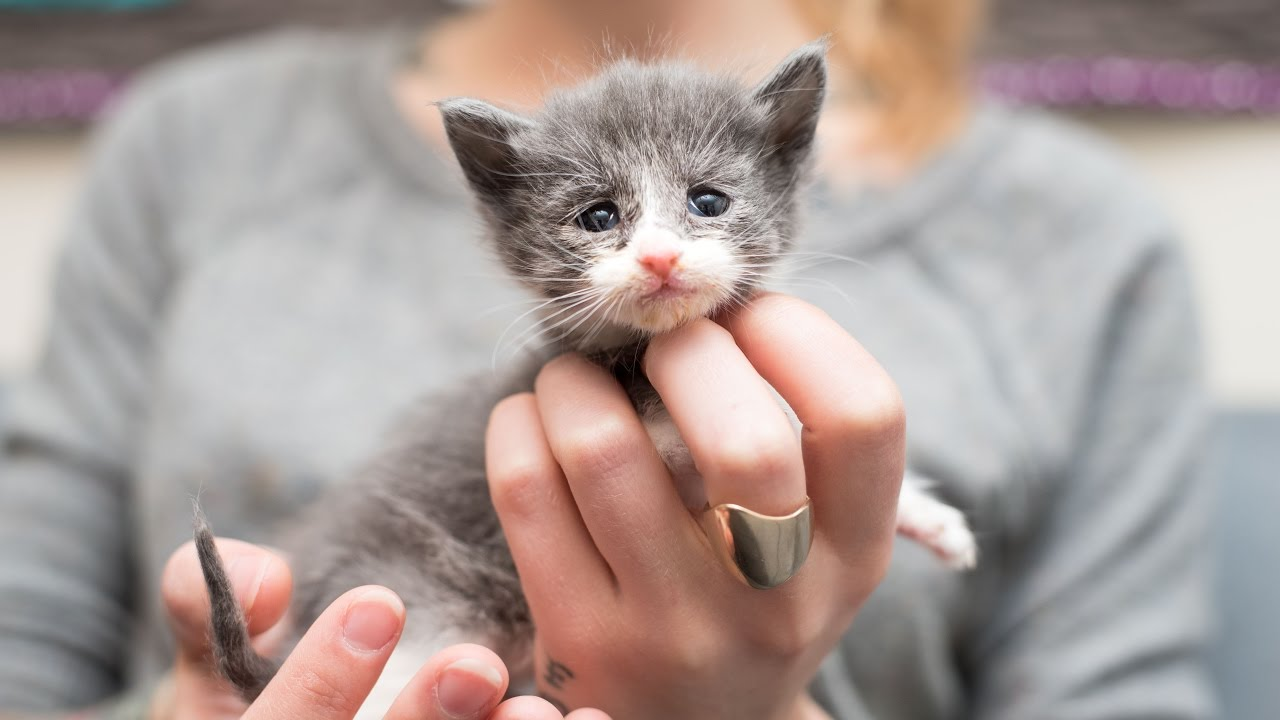
\includegraphics[width=0.5\textwidth]{Pictures/kitten-placeholder.jpg}
%\caption{Scenario 1. Timestep smaller than 1/4 of fluctuation period}
%\label{time1}
%\end{figure}

%\textbf{Scenario 2:} timestep is equal to the  1/4 of the fluctuation period (Fig. \ref{time2}).

%\begin{figure}[h!]
%\centering % bo \centering nie wstawia dodatkowego odstępu
%%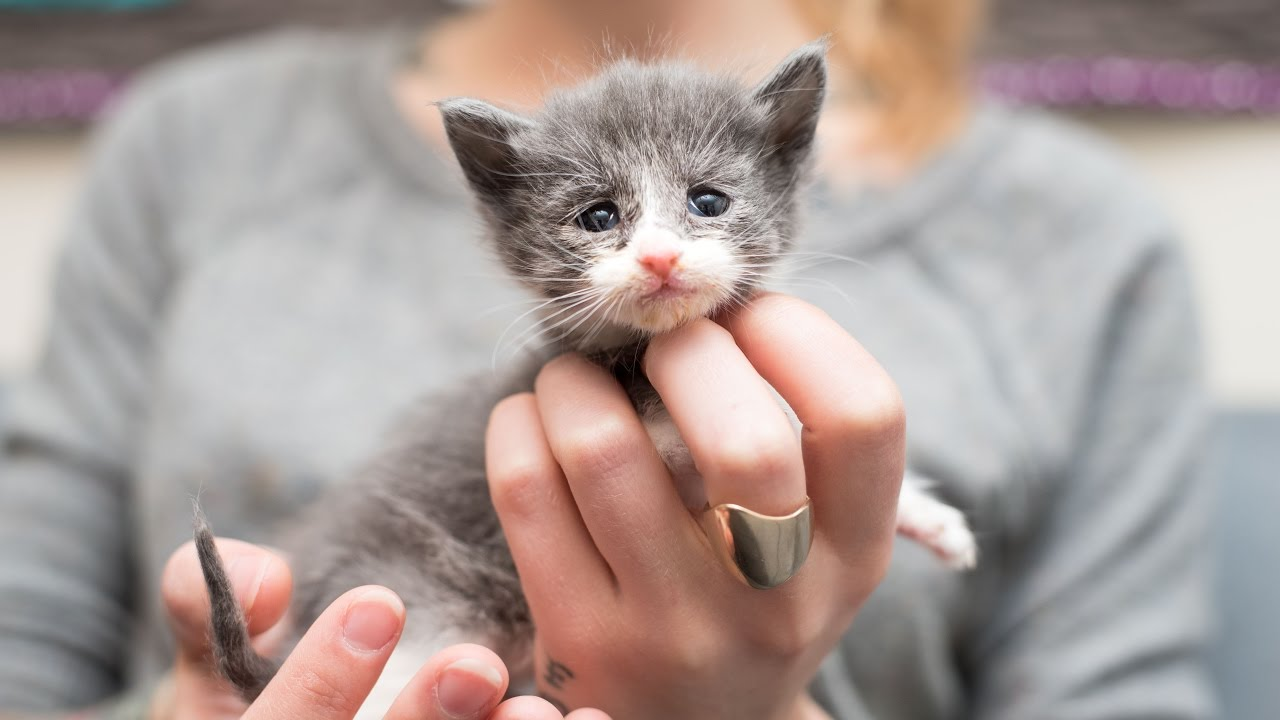
\includegraphics[width=0.5\textwidth]{Pictures/kitten-placeholder.jpg}
%\caption{Scenario 2. Timestep equal to 1/4 of fluctuation period}
%\label{time2}
%\end{figure}

%\textbf{Scenario 3:} timestep is equal to fluctuation period (Fig. \ref{time3}).

%\begin{figure}[h!]
%\centering % bo \centering nie wstawia dodatkowego odstępu
%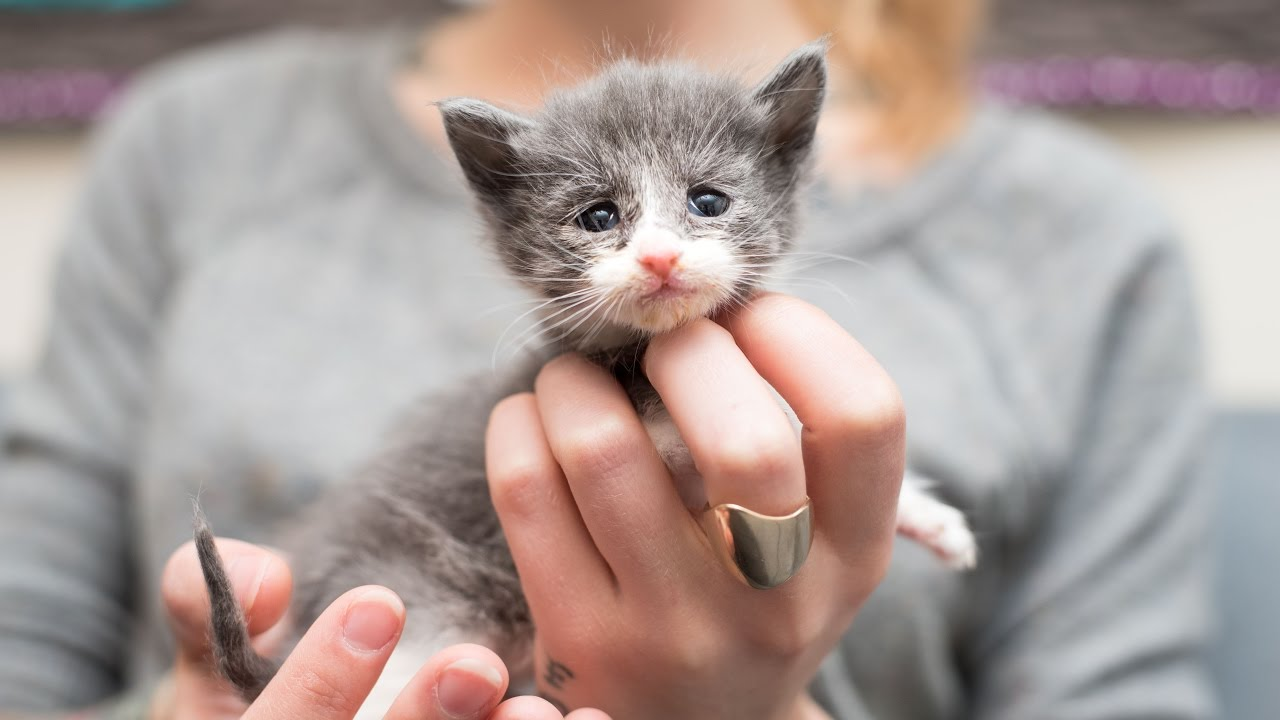
\includegraphics[width=0.5\textwidth]{Pictures/kitten-placeholder.jpg}
%\caption{Scenario 3. Timestep equal to fluctuation period}
%\label{time3}
%\end{figure}

%\textbf{Scenario 4:} timestep is larger that fluctuation period (Fig. \ref{time4}).

%\begin{figure}[h!]
%\centering % bo \centering nie wstawia dodatkowego odstępu
%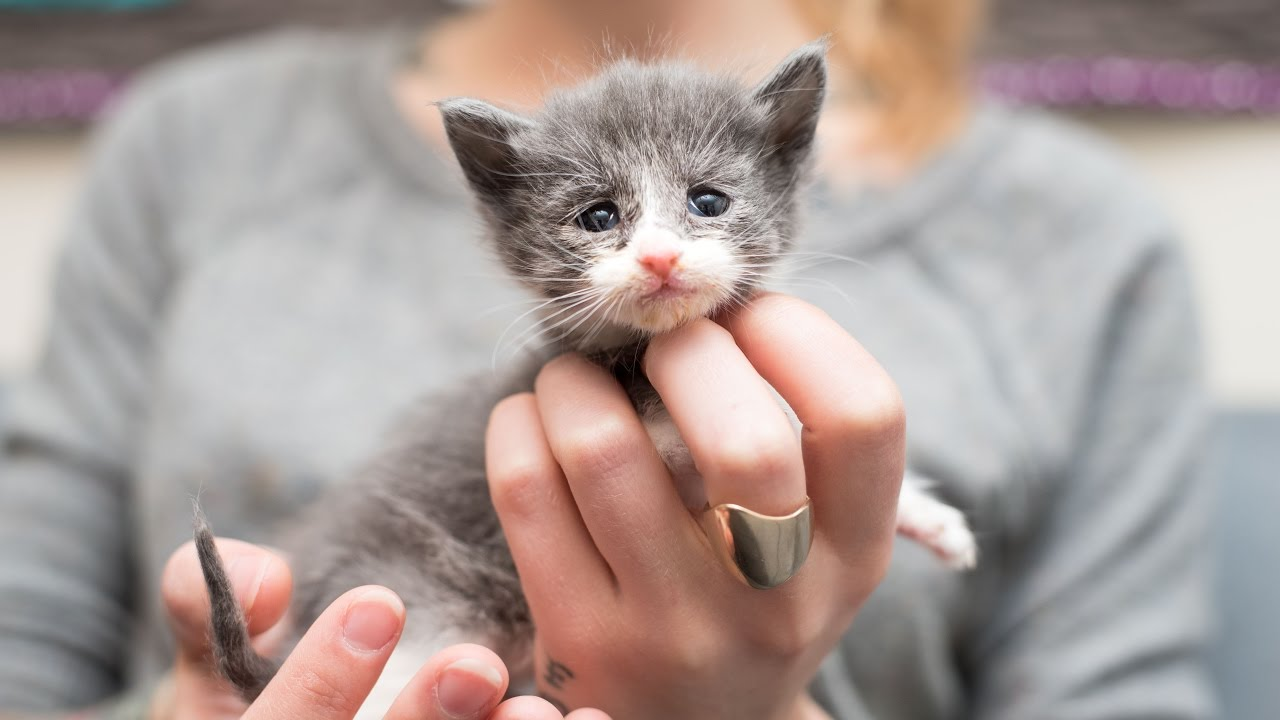
\includegraphics[width=0.5\textwidth]{Pictures/kitten-placeholder.jpg}
%\caption{Scenario 4. Timestep is larger than fluctuation period}
%\label{time4}
%\end{figure}
%\end{itemize}

In order to capture frequencies on the low end of the spectrum, the analysis must be performed long enough to capture at least a single, with optimum 5 or more periods, of the desired low frequency. Assuming lower end of the audible frequency spectrum, the 20Hz frequency, the simulation time must resemble at least 0.05s of flow time with optimum 0.25s of flow time at given timestep.


%----------------------------------------------------------------------------------------
%	SECTION
%----------------------------------------------------------------------------------------
\section{Limiting factors of the direct approach} \label{limits}
Described direct formulation noise analysis is solely a post processing approach relying on data generated on CFD analysis. In order to obtain reasonable results down the process, the analysis itself mus be capable of delivering pressure fluctuations that can be considered as acoustic in source. 

It is advised to used a turbulence model that is capable of resolving small scale turbulence on a mesh that will allow such resolution. Utilizing LES formulation or at least hybrid RANS/LES turbulence model such as DDES. Using an averaging formulation such as RANS will cut off all of the fluctuations and is not suitable for this approach.

%Pressure signal used by this approach is given by a list of real scalar values for each node or cell centroid for each timestep. Therefore obtaining phase shift of the ordinary sinuses components of pressure signal may be challenging, if at all possible, and relies solely on further postprocessing of generated data. 

The range of frequencies captured by this method depends on the mesh sizing and timestep sizing. Therefore, if the range of expected frequencies is known or at least estimated, the mesh sizing and timestep size can be adjusted for the given case. For analysis within audible range, 4000 timesteps are required for one 20Hz period. Considering the mesh sizing requirements, the mesh cell count will rise up to tens of millions for a single passage axial compressor blade. This makes the case files and storing data for each timestep relatively challenging and requires securing adequate storage beforehand.
 
A major limiting factor is the implementation of the direct noise formulation post-processing. For this thesis, the method was implemented in python v.3.5 high level programming language. Python code is written in C/C++ and provides a vast array of additional libraries for handling files, tabular data and performing mathematical operations. The code is presented in appendices to this dissertation. Although easy to implement, python code is known to be inefficient and slow while managing large amounts of data. Tools and algorithms used in implementing the averaging, obtaining sound pressure and particle velocity as well as DFT are build in tools from specific libraries. As convenient for the implementation, the post-processing code requires some amount of operational memory and disk space for generating the results.

The programming language used for the post-processing of data must be capable of generating 2D and 3D plots for visualization purposes. Ideally the processed and visualized data should resemble the mesh from which the initial data was gathered.
